\documentclass[tikz,border=10pt]{standalone}
\usetikzlibrary{arrows.meta,positioning,decorations.pathreplacing}
\usepackage{amssymb}
\usepackage{xcolor}
\pagecolor{white}
\begin{document}
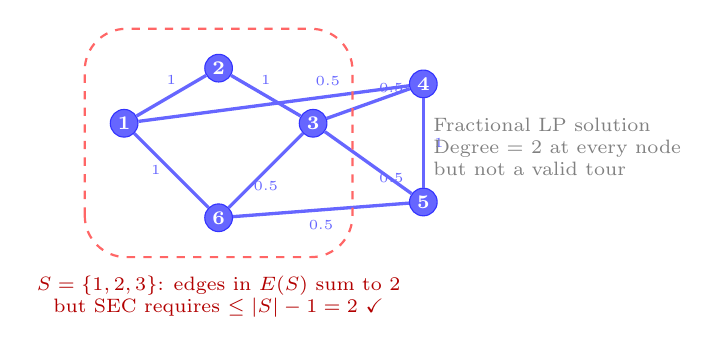
\begin{tikzpicture}[
  city/.style={circle, draw=blue!80, fill=blue!60, inner sep=0pt,
               minimum size=10pt, font=\scriptsize\bfseries, text=white},
  edge/.style={very thick},
  cut/.style={thick, red!60, dashed},
]
  % Cities
  \node[city] (1) at (0, 1.5)   {1};
  \node[city] (2) at (1.2, 2.2) {2};
  \node[city] (3) at (2.4, 1.5) {3};
  \node[city] (4) at (3.8, 2)   {4};
  \node[city] (5) at (3.8, 0.5) {5};
  \node[city] (6) at (1.2, 0.3) {6};

  % Edges with fractional values
  \draw[edge, blue!60] (1) -- node[above, font=\tiny] {1} (2);
  \draw[edge, blue!60] (2) -- node[above, font=\tiny] {1} (3);
  \draw[edge, blue!60] (3) -- node[above right, font=\tiny] {0.5} (4);
  \draw[edge, blue!60] (3) -- node[below right, font=\tiny] {0.5} (5);
  \draw[edge, blue!60] (4) -- node[right, font=\tiny] {1} (5);
  \draw[edge, blue!60] (5) -- node[below, font=\tiny] {0.5} (6);
  \draw[edge, blue!60] (6) -- node[left, font=\tiny] {1} (1);
  \draw[edge, blue!60] (4) -- node[above, font=\tiny, pos=0.3] {0.5} (1);
  \draw[edge, blue!60] (6) -- node[below, font=\tiny] {0.5} (3);

  % SEC violation region
  \draw[cut, rounded corners=15pt]
    (-0.5, -0.2) rectangle (2.9, 2.7);

  \node[font=\scriptsize, red!70!black, align=center] at (1.2, -0.7)
    {$S = \{1,2,3\}$: edges in $E(S)$ sum to $2$\\but SEC requires $\leq |S|-1 = 2$ \checkmark};

  \node[font=\scriptsize, gray, align=left] at (5.5, 1.2)
    {Fractional LP solution\\Degree = 2 at every node\\but not a valid tour};
\end{tikzpicture}
\end{document}
